\chapter{Development of Balance System}

\section{Development of module through OOP, managing models and controllers}

\subsection{Balance Updates}

\subsubsection{UML}

\subsubsection{Balance Updates Status}

\begin{figure} [h!]
    \centering
    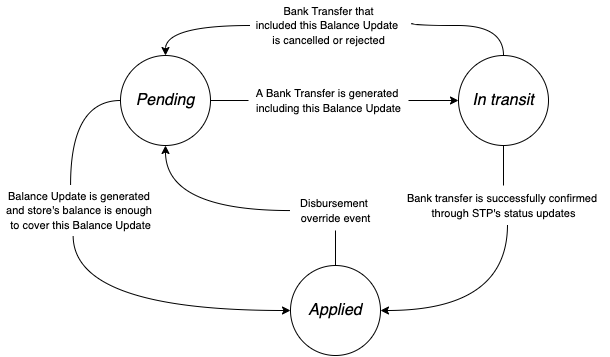
\includegraphics[scale = 0.7]{assets/diagrams/BalanceUpdatesStateMachine.png}
    \caption{Balance Updates State Machine}\label{fig:state_machine_balance_updates}
\end{figure}

\subsubsection{Balance Updates Types}

\subsubsection{Overwriting Balance Updates}


Balance Updates have an attribute to indicate if the object was overwritten. Whenever an object is overwritten, this means that there is an additional Balance Update that is cancelling its affectation on the store’s general balance. This is particularly helpful to keep control of a store’s balance modification for those Balance Updates that are generated with the status of Applied. The only Balance Updates that could be overwritten are those of the types of Disbursement and Contribution. 
A Balance Update of type Disbursement is generated whenever a confirmation that a Bank Transfer has been successfully accepted by the receiving party is received. There is a very particular edge case where the money could be returned even after it was confirmed. For these cases, the Disbursement that was generated is no longer valid, hence, an update to the store’s balance should be made. This is done by generating an additional Balance Update with type Disbursement Override. This new Balance Update will contribute once again the amount that was marked as disbursed to the store’s balance.
Furthermore, Balance Updates of type Contribution could also be overwritten at some point. These are created once a partner has confirmed a product’s delivery through their dashboard and the credit of that product will generate a contribution to the store’s balance. This means that there is some amount that Atrato must eventually transfer to the partner’s bank account depending on the disbursement modality that this partner has active. These contributions could eventually be overwritten if the credit is later cancelled, which may happen at some points for external reasons. For this particular scenario, a new Balance Update of type Credit cancelation needs to be created to compensate the previous contribution, regardless of the contribution’s status as shown in Figure \ref{fig:dlowchart_credit_cancelation}.

\begin{figure} [h]
    \centering
    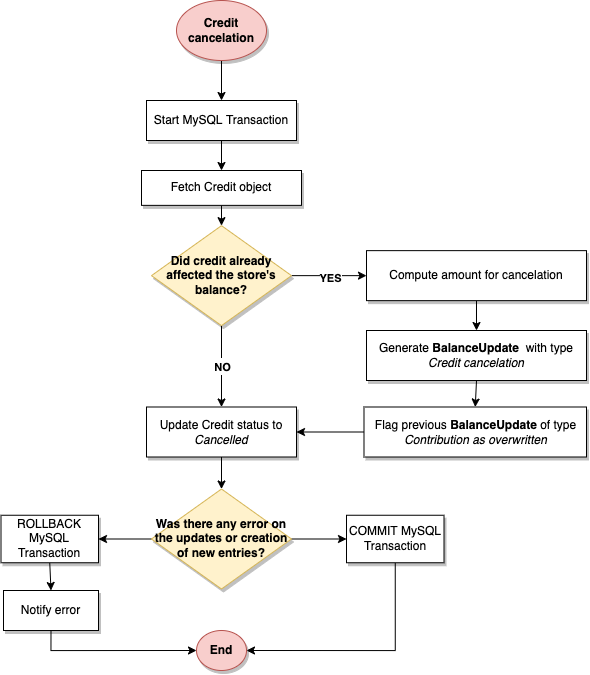
\includegraphics[scale = 0.7]{assets/flowcharts/CreditCancelation.png}
    \caption{Processing a credit's cancelation and its affectation to a store's balance system}\label{fig:dlowchart_credit_cancelation}
\end{figure}

\section{Ensure correct functionality and error handling through MySQL Transactions}

\section{Detailed visibility and traceability of full process}

\subsection{Implementation of existing Logging system}

\section{Security through implementation of existing IAM Module}

\section{Manual implementation of automation}
